\documentclass[lettersize,journal]{IEEEtran}
\usepackage{amsmath,amsfonts}
\usepackage{algorithmic}
\usepackage{algorithm}
\usepackage{array}
\usepackage[caption=false,font=normalsize,labelfont=sf,textfont=sf]{subfig}
\usepackage{textcomp}
\usepackage{stfloats}
\usepackage{url}
\usepackage{verbatim}
\usepackage{graphicx}
\usepackage{cite}
\usepackage[center]{caption}
\hyphenation{op-tical net-works semi-conduc-tor IEEE-Xplore}

\begin{document}

\title{Lab 1 - Edge Detectors \\ \vspace{0.1em} \LARGE Computational Vision \& Imaging}

\author{\textbf{Student ID}: XXXXXXX \\
~\IEEEmembership{Random Student,~School of Computer Science,\\University of Birmingham, UK, B15 2TT}
% <-this % stops a space
\thanks{This is a solution for the Formative Assignment by Hamid Dehghani}
% <-this % stops a space
\thanks{The report was submitted to Canvas on Feb 19 and reviewed by a TA}}

% The paper headers
\markboth{Collection of Lab Reports, Computer Vision, No.~1, February~2022}%
{Shell \MakeLowercase{\textit{et al.}}: A collection of Report submissions documenting assignment solutions}

\maketitle

\begin{abstract}
This document is a formal solution for the Lab 1 Formative Assignment based on the Edge Detection. It explains the difference between using \emph{Sobel} and \emph{Roberts} filters when identifying image edges as well as shows the impact of different thresholds and what happens when the magnitude function is approximated.
\end{abstract}

\begin{IEEEkeywords}
Lab 1, formative assignment, computer vision, imaging, edge detection, filters, kernels, Sobel, Robert, MATLAB.
\end{IEEEkeywords}

\section{Introduction}
\IEEEPARstart{D}{uring} the lectures we were shown that an image can be represented as a matrix of intensity values, a so called \textbf{intensity image}. By evaluating how the intensity changes throughout the image pixels, we are able to determine where the biggest variations occur, thus signaling where a potential edge can be present. Such technique is a powerful way to detect the region changes in the image while reducing the amount of data but preserving the structural properties.

\section{Setup}
We are given an image "shakey.150.gif" (\ref{fig:1}) on which we need to apply edge detection filters.

\begin{figure}[h]
    \centering
    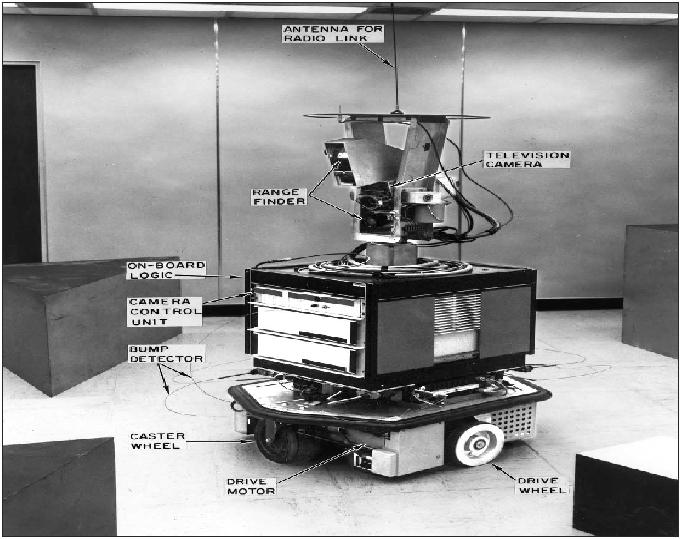
\includegraphics[height=15em]{figures/shakey150.jpg}
    \caption{grey-scale "Shakey 150" image}
    \label{fig:1}
\end{figure}

We are also given 2 MATLAB files "sobel.mat" and "roberts.mat" each containing horizontal and vertical weight matrices for calculating gradients at local regions in the image. The \emph{Sobel} kernels can be seen in equation \ref{eq:1} and the \emph{Roberts} kernels in equation \ref{eq:2}.

\begin{equation}
    \label{eq:1}
    \text{SobelX} = \begin{bmatrix} -1 & 0 & 1 \\ -2 & 0 & 2 \\ -1 & 0 & 1 \end{bmatrix};\ 
    \text{SobelY} = \begin{bmatrix} -1 & -2 & -1 \\ 0 & 0 & 0 \\ 1 & 2 & 1 \end{bmatrix}
\end{equation}

\begin{equation}
    \label{eq:2}
    \text{RobertsA} = \begin{bmatrix} 1 & 0 \\ 0 & -1 \end{bmatrix};\ 
    \text{RobertsB} = \begin{bmatrix} 0 & 1 \\ -1 & 0 \end{bmatrix}
\end{equation}

If we convolve the image with these filters (we already assume the filters are flipped, otherwise it is a \emph{cross-correlation}), we get a different map for each filter. If we apply a threshold, we can see exactly which pixels "pass the criteria" for being considered as an edge. This can be seen in figure \ref{fig:2} where a threshold of 60 was used for \emph{Sobel} maps and a threshold of 20 for \emph{Roberts} maps.

\begin{figure}[h]
    \centering
    \begin{tabular}{cccc}
        \subfloat[Sobel horizontal]{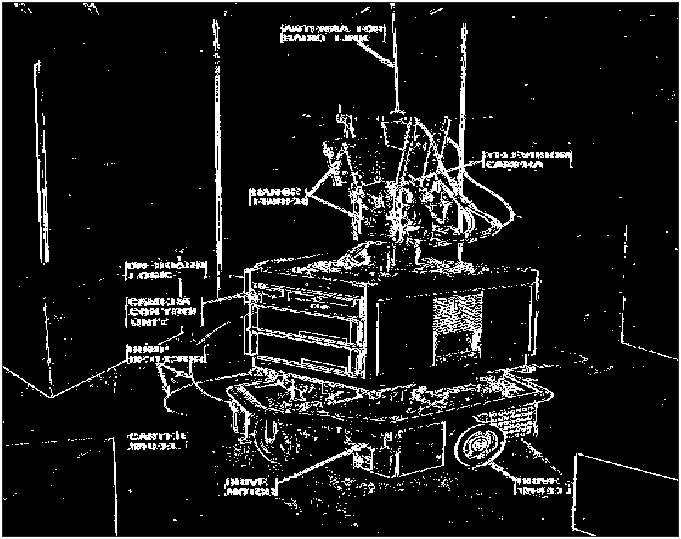
\includegraphics[width = 1.55in]{figures/sobel_horizontal.jpg}} &
        \subfloat[Sobel vertical]{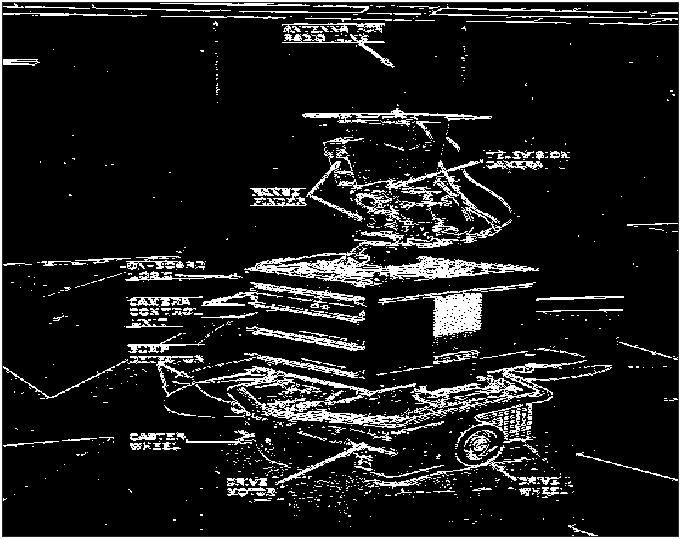
\includegraphics[width = 1.55in]{figures/sobel_vertical.jpg}}\\
        \subfloat[Roberts horizontal]{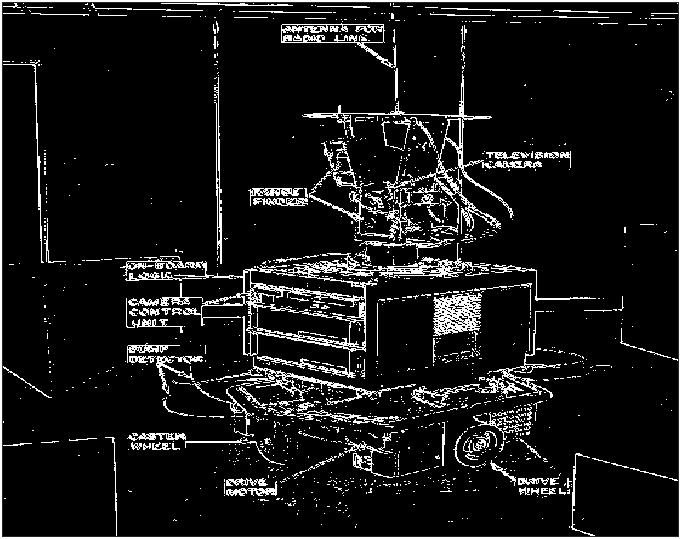
\includegraphics[width = 1.55in]{figures/roberts_horizontal.jpg}} &
        \subfloat[Roberts vertical]{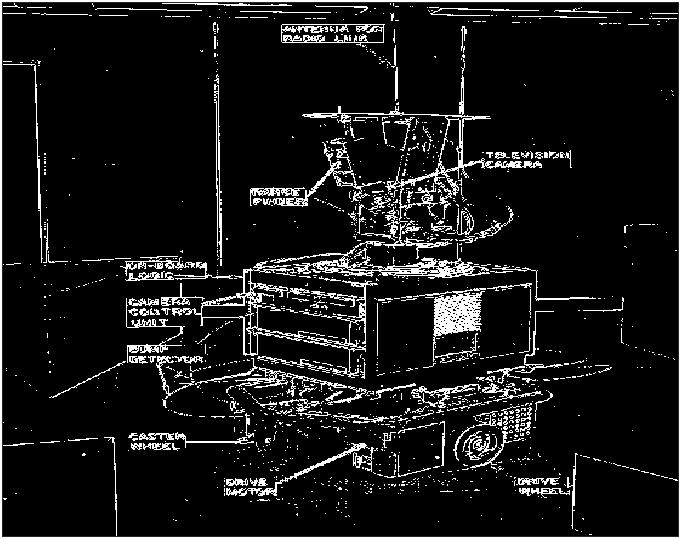
\includegraphics[width = 1.55in]{figures/roberts_vertical.jpg}}
    \end{tabular}
    \caption{filter maps after convolving edge kernels with the image}
    \label{fig:2}
\end{figure}

\section{Methodology}

Before we get into tasks, we need to define certain methods on which the experiments/findings depend on in section \ref{Tasks}. We know that if we compute the gradient in x direction $\nabla_x G$ and in y direction $\nabla_y G$, we can compute the total magnitude by applying Pythagorean theorem. The acquired \textbf{intensity map} can be seen in figure \ref{fig:3} - \emph{Sobel} map is more clear as it has higher weights towards the centre filter than \emph{Roberts}.

\begin{figure}[ht]
    \centering
    \begin{tabular}{cccc}
        \subfloat[Sobel map]{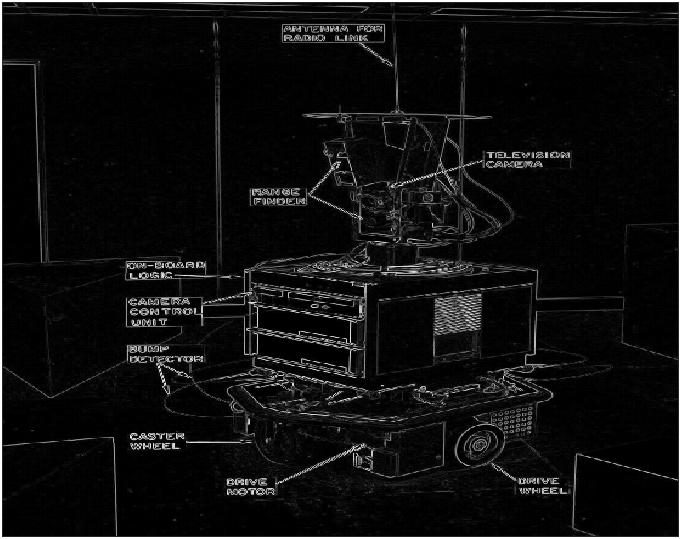
\includegraphics[width = 1.55in]{figures/sobel_no_thres.jpg}} &
        \subfloat[Roberts map]{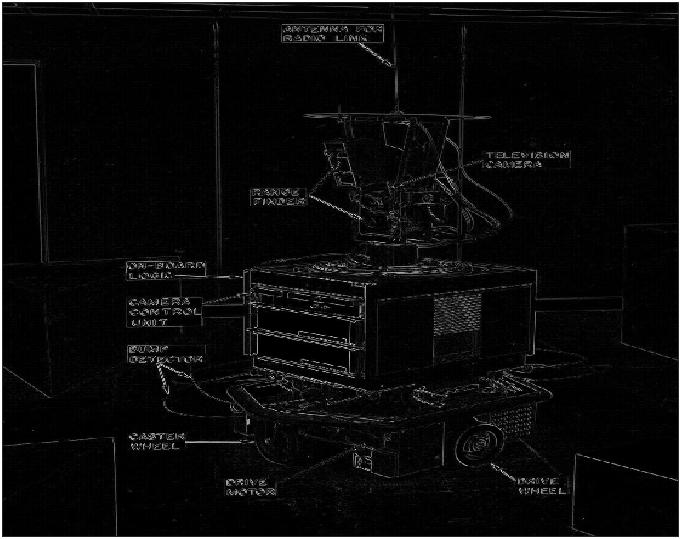
\includegraphics[width = 1.55in]{figures/roberts_no_thres.jpg}}
    \end{tabular}
    \caption{non-thresholded magnitude maps}
    \label{fig:3}
\end{figure}

The computation for the exact magnitude can be seen in formula \ref{eq:3} but we can also approximate the magnitude using formula \ref{eq:4}.

\begin{equation}
    \label{eq:3}
    \text{magnitude} = \sqrt{\nabla_x G^2 + \nabla_y G^2}
\end{equation}
\begin{equation}
    \label{eq:4}
    \text{magnitude\_approximation} = |\nabla_x G| + |\nabla_y G|
\end{equation}

As well as computing the magnitudes, we will need to compute the absolute and the relative errors to compare how similar the approximate magnitude is to the exact magnitude. Absolute error can be found by equation \ref{eq:5} and the relative error by \ref{eq:6} if we compare true value $x$ and predicted value $\hat x$.

\begin{equation}
    \varepsilon_{\text{abs}} = |x - \hat x|
    \label{eq:5}
\end{equation}

\begin{equation}
    \varepsilon_{\text{rel}} = \frac{\varepsilon_{\text{abs}}}{|x|}
    \label{eq:6}
\end{equation}
\\
For matrices, we just compute the average over all entries.

\section{Tasks} \label{Tasks}
\subsection{Task 1}

\noindent\textbf{Question 1}: What do you notice regarding the effect of changing the threshold? \\

\noindent\textbf{Answer 1}: The smaller the threshold, the more noise and the more details there are in the image. The bigger the threshold, the less noise and the less details there are.\\

What happens with a low threshold is that we allow even relatively small values to be identified as image edges, and since at least some amount of the rate of change in intensity is present even in plain areas (due to noise), we get lots of pixels identified as edges. In contrast, with high threshold, we care only about the biggest changes in intensity, therefore, only the major contours are identified, leaving out most of the noise and minor edges undetected. In general, we can see a trade-off between image noise and contour smoothness.\\

This can be witnessed in figure \ref{fig:4} where 4 different \emph{Sobel} magnitude maps show how increasing the threshold diminishes the high value (white) pixels in the image (i.e., edges or potential edges).

\begin{figure}[ht]
    \centering
    \begin{tabular}{cccc}
        \subfloat[$t=10$]{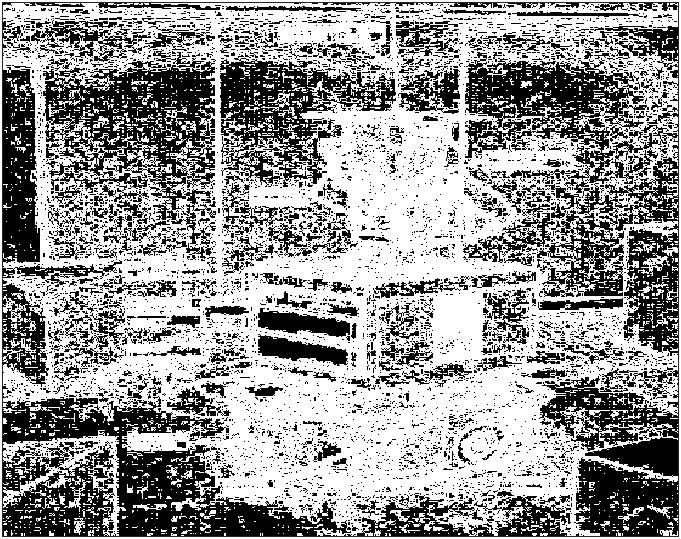
\includegraphics[width = 1.55in]{figures/sobel_10.jpg}} &
        \subfloat[$t=40$]{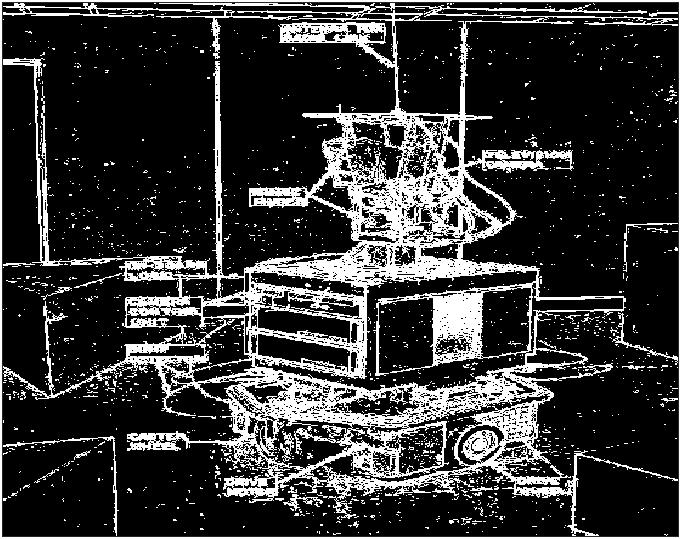
\includegraphics[width = 1.55in]{figures/sobel_40.jpg}}\\
        \subfloat[$t=70$]{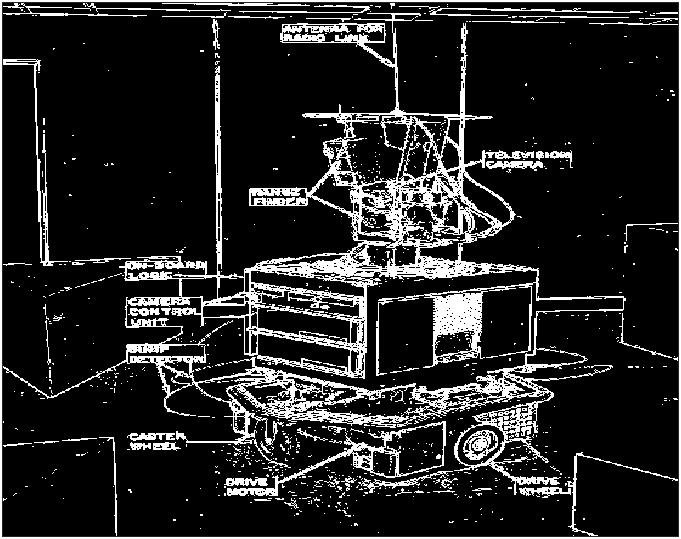
\includegraphics[width = 1.55in]{figures/sobel_70.jpg}} &
        \subfloat[$t=100$]{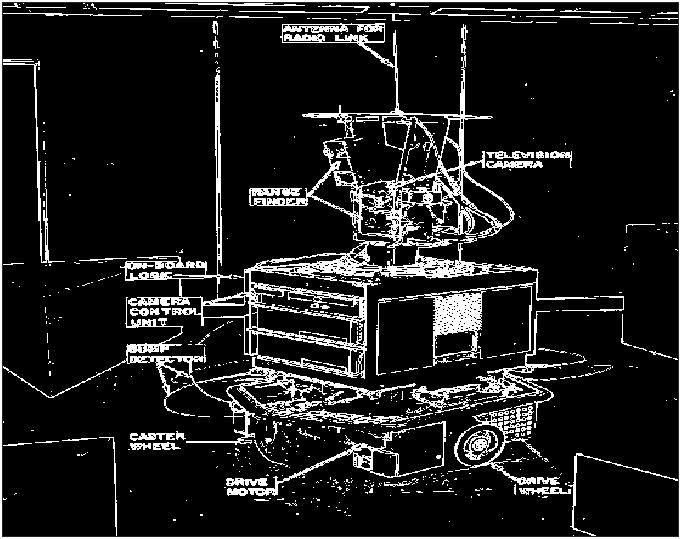
\includegraphics[width = 1.55in]{figures/sobel_100.jpg}}
    \end{tabular}
    \caption{Sobel magnitude maps after applying different thresholds}
    \label{fig:4}
\end{figure}

\subsection{Task 2}

\noindent\textbf{Question 2}: What do you notice regarding the difference between Sobel and Roberts?\\

\noindent\textbf{Answer 2}: Using Roberts filters, the contours are identified with relatively low thresholds, for example, with threshold 20, strong edges are detected and some small ones are even undetected, meaning 20 is slightly too high to capture small details. However, there is more noise too, so the trade-off is more overlapping compared to the trade-off when using Sobel filters.\\

The magnitude maps acquired by applying Robets filter with different thresholds can be seen in figure \ref{fig:5}.

\begin{figure}[ht]
    \centering
    \begin{tabular}{cccc}
        \subfloat[$t=5$]{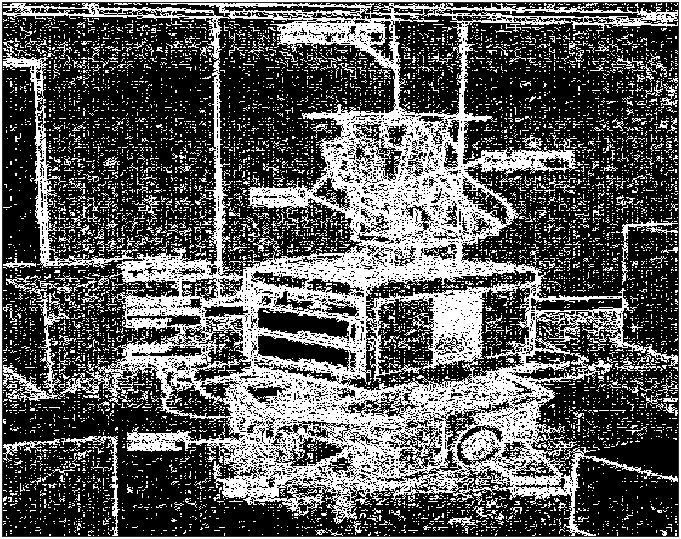
\includegraphics[width = 1.55in]{figures/roberts_5.jpg}} &
        \subfloat[$t=10$]{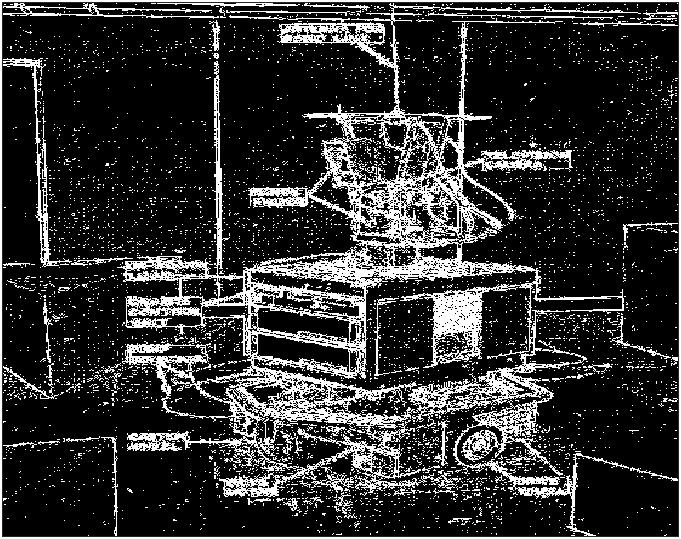
\includegraphics[width = 1.55in]{figures/roberts_10.jpg}}\\
        \subfloat[$t=15$]{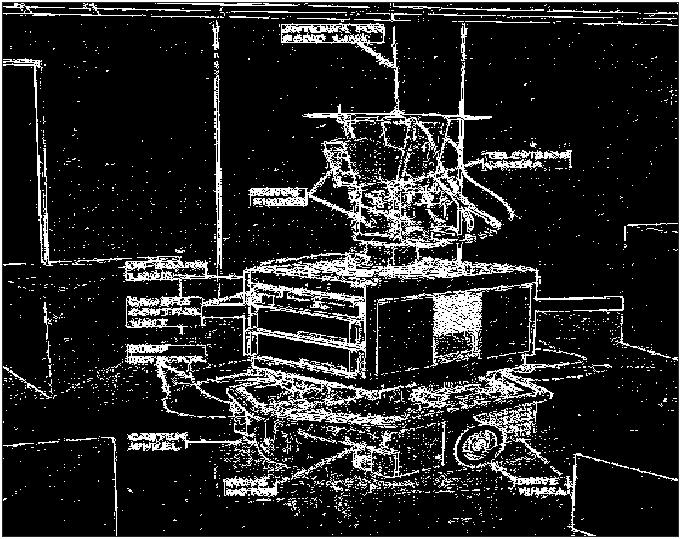
\includegraphics[width = 1.55in]{figures/roberts_15.jpg}} &
        \subfloat[$t=20$]{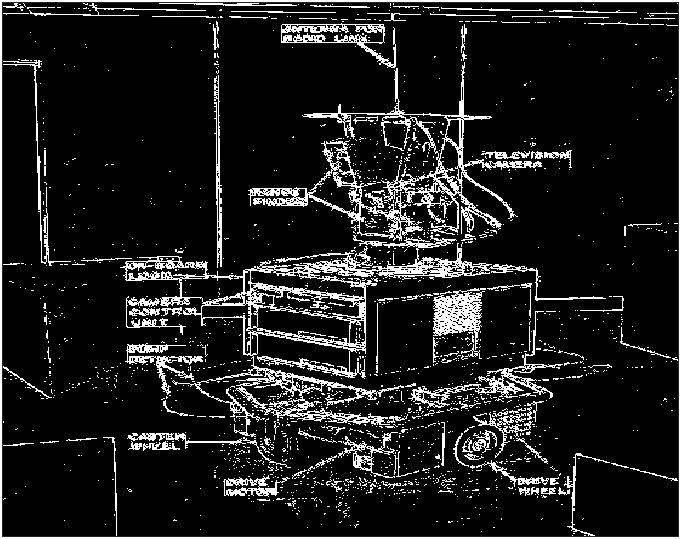
\includegraphics[width = 1.55in]{figures/roberts_20.jpg}}
    \end{tabular}
    \caption{Roberts magnitude maps after applying different thresholds}
    \label{fig:5}
\end{figure}

 As we can see, compared with Sobel maps, more noise is present even for higher threshold values. This happens because we compute the gradients at local regions of size 2-by-2 which is more sensitive than when we calculate gradients at 3-by-3 regions because we don't take into account the surrounding pixels which provide more generalized information about the rate of change of intensity in that region and smoothen the gradient.

\subsection{Task 3}

\noindent\textbf{Question 3}: What do you notice regarding the difference between magnitude and absolute when calculating the edge?\\

\noindent\textbf{Answer 3}: When using absolute values we introduce more noise because there is an approximation error (for example, in the case of using Roberts filters the relative error is ~31.48\%). However less time is taken to calculate the absolute measure than the exact magnitude (for example, in the case of using Sobel filters, the absolute measure is calculated 3-6 times faster than the magnitude). However, the result is still similar and, if efficiency is required, the absolute measure could be used as a substitute for the exact magnitude measure.\\

The example of maps acquired through magnitude approximation can be seen in figure \ref{fig:6}. It is noticable that the samples contain more noise than when computing the exact magnitudes, such as in figures \ref{fig:4}, \ref{fig:5}.

\begin{figure}[ht]
    \centering
    \begin{tabular}{cccc}
        \subfloat[$t=40$]{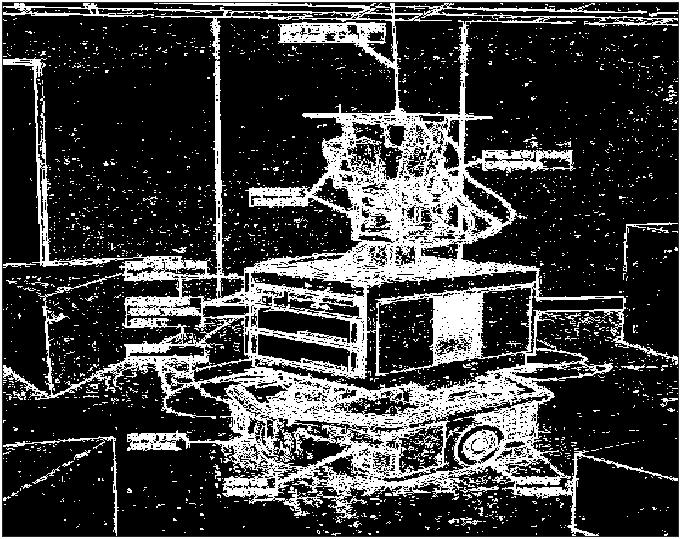
\includegraphics[width = 1.55in]{figures/sobel_40_approx.jpg}} &
        \subfloat[$t=70$]{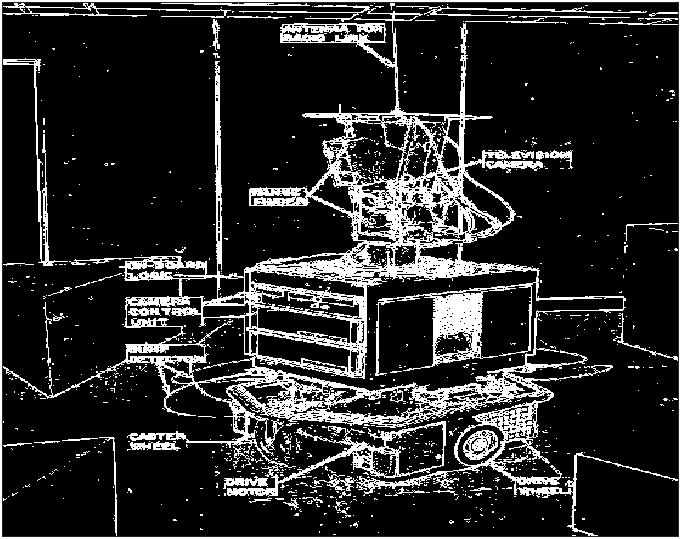
\includegraphics[width = 1.55in]{figures/sobel_70_approx.jpg}}\\
        \subfloat[$t=10$]{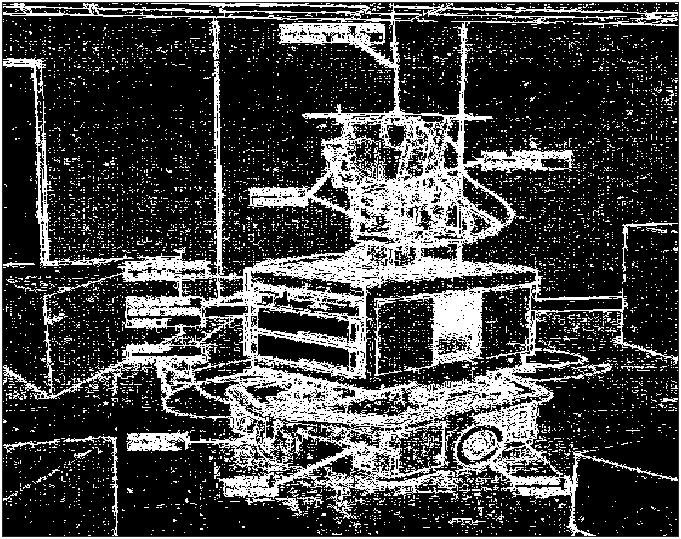
\includegraphics[width = 1.55in]{figures/roberts_10_approx.jpg}} &
        \subfloat[$t=15$]{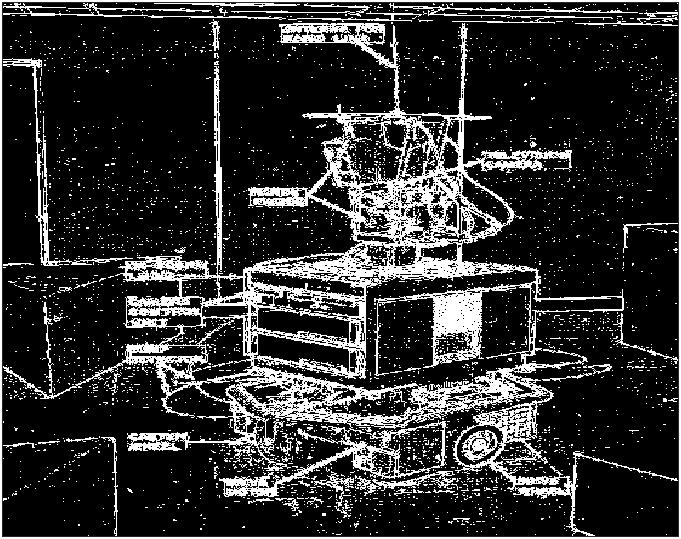
\includegraphics[width = 1.55in]{figures/roberts_15_approx.jpg}}
    \end{tabular}
    \caption{Sobel (upper row) and Roberts (lower row) maps after applying magnitude approximation on different thresholds}
    \label{fig:6}
\end{figure}

\begin{thebibliography}{1}
\bibliographystyle{IEEEtran}

\bibitem{ref1}
Sobel, Irwin. (2014). {\it{An Isotropic 3x3 Image Gradient Operator}}. Presentation at Stanford A.I. Project 1968. 

\bibitem{ref2}
LS. Davis, "A survey of edge detection techniques", Computer Graphics and Image Processing, vol 4, no. 3, pp 248-260, 1975.

\end{thebibliography}
\vfill
\end{document}